% thesis.tex
%
% Enjoy, evolve, and share!
%
% Compile it as follows:
% xelatex demo.tex
% bibtex demo.aux
% xelatex demo.tex && xelatex demo.tex
%
% Alternatively, compile it using `make -i' (see the provided Makefile).
%
% Check file `dimscthesis.cls' for other configuration options.
%
%
% This documentclass supports the following options:
% en
% 		If present, the document adds some English pages in the front matter
% 		plus changes some headings to English. Use this option if thesis is in English.
%       Omit if written in Greek.
%
% inscr
% 		If present, then a page with the inscription provided via the command
% 		\inscription{} is printed.
%
% ack
%		If present, then a page with the acknowledgements provided via the
%		command \acksEn{} is printed.
%
% preface
%		If present, then a preface page is included just before the
%		introductory chapter. The content of this page is controled via the
%		command \preface{}.
%
% oneside
%		If present, the thesis is formatted as if it will be printed on
%		only one side of each page, the other side being left blank.
%		Default is "twoside", which is used when this option is omitted.
%
\documentclass[en,inscr,ack,preface]{dimscthesis}

% Scans for figures relative to this file
\graphicspath{ {./figures/} }

%%%%%%%%%%%%%%%%%%%%%%%%%%%%%%%%%%%%%%%%%%%%%%%%%%%%%%%%%%%%%%%%%%%%%%%%%%%%%%%
%%%%%%%%%%%%%%%%%%%% User-specific package inclusions %%%%%%%%%%%%%%%%%%%%%%%%%
%%%%%%%%%%%%%%%%%%%%%%%%%%%%%%%%%%%%%%%%%%%%%%%%%%%%%%%%%%%%%%%%%%%%%%%%%%%%%%%
\hypersetup{
    unicode=true,                     % non-Latin characters in bookmarks
    pdffitwindow=true,                % page fit to window when opened
    pdfnewwindow=true,                % links in new window
    pdfkeywords={list, of, keyword},  % list of keywords
    colorlinks=true,                  % false: boxed links; true: colored links
    linkcolor=black,                  % color of internal links
    citecolor=black,                  % color of links to bibliography
    filecolor=black,                  % color of file links
    urlcolor=black,                   % color of external links
    pdftitle={Thesis title},          % title
    pdfauthor={Laertis Moustakas},    % author
    pdfsubject={Thesis}               % subject of the document
}
\urlstyle{same}
%%%%%%%%%%%%%%%%%%%%%%%%%%%%%%%%%%%%%%%%%%%%%%%%%%%%%%%%%%%%%%%%%%%%%%%%%%%%%%%
%%%%%%%%%%%%%%%%%%%% User-specific package inclusions %%%%%%%%%%%%%%%%%%%%%%%%%
%%%%%%%%%%%%%%%%%%%%%%%%%%%%%%%%%%%%%%%%%%%%%%%%%%%%%%%%%%%%%%%%%%%%%%%%%%%%%%%
\usepackage[shortlabels]{enumitem}
\usepackage{lscape}
\usepackage{subcaption}
\usepackage{listings}

%%%%%%%%%%%%%%%%%%%%%%%%%%%%%%%%%%%%%%%%%%%%%%%%%%%%%%%%%%%%%%%%%%%%%%%%%%%%%%%
%%%%%%%%%%%%%%%%%%%%%% User-specific configuration %%%%%%%%%%%%%%%%%%%%%%%%%%%%
%%%%%%%%%%%%%%%%%%%%%%%%%%%%%%%%%%%%%%%%%%%%%%%%%%%%%%%%%%%%%%%%%%%%%%%%%%%%%%%

%%%%%%%%%%%%%%%%%%%%%%%%%%%%%%%%%%%%%%%%%%%%%%%%%%%%%%%%%%%%%%%%%%%%%%%%%%%%%%%
%%%%%%%%%%%%%%%%%%%%%%%%%%% Required Metadata %%%%%%%%%%%%%%%%%%%%%%%%%%%%%%%%%
%%%%%%%%%%%%%%%%%%%%%%%%%%%%%%%%%%%%%%%%%%%%%%%%%%%%%%%%%%%%%%%%%%%%%%%%%%%%%%%
%
% First name, last name
%
\authorFirstGr{Όνομα}
\authorFirstAbrGr{Ο.} % abbreviation of first name
\authorMiddleGr{Μ.}   % abbreviation of father's first name
\authorLastGr{Επώνυμο}
\authorFirstEn{First}
\authorFirstAbrEn{F.}
\authorMiddleEn{M.}
\authorLastEn{Last}
\authorSN{DSXXXXXXX}

%
% Program (greek and english)
%
\programGr{ΤΙΤΛΟΣ ΠΡΟΓΡΑΜΜΑΤΟΣ ΜΕΤΑΠΤΥΧΙΑΚΩΝ ΣΠΟΥΔΩΝ}
\programEn{POSTGRADUATE MASTERS PROGRAM TITLE}

%
% The title of the thesis
%
\titleGr{Τίτλος Διπλωματικής Εργασίας}
\titleEn{Postgraduate Thesis Title}

%
% Month followed by Year
%
\dateGr{ΟΚΤΩΒΡΙΟΣ 2023}
\dateEn{OCTOBER 2023}

%
% Advisor info
%
\advisorGr{Επιβλέπων Πρώτος}
\advisorRankGr{Καθηγητής}
\advisorOrgGr{ΕΚΠΑ}
\advisorEn{Board First}
\advisorRankEn{Professor}
\advisorOrgEn{NKUA}

%
% Members of the advisory board
% (the first one, will be automatically taken up by the advisor)
%
\boardTwoGr{Επιβλέπων Δεύτερος}
\boardTwoRankGr{Καθηγητής}
\boardTwoOrgGr{ΕΚΠΑ}
\boardTwoEn{Board Second}
\boardTwoRankEn{Professor}
\boardTwoOrgEn{NKUA}

\boardThreeGr{Επιβλέπων Τρίτος}
\boardThreeRankGr{Καθηγητής}
\boardThreeOrgGr{ΕΚΠΑ}
\boardThreeEn{Board Third}
\boardThreeRankEn{Professor}
\boardThreeOrgEn{NKUA}

%
% The examination date of the thesis
%
\examinationDateGr{1 Οκτωβρίου 2023}
\examinationDateEn{1 October, 2023}

%
% Supervisors[heading(optional, defaluts to ΕΠΙΒΛΕΠΩΝ/SUPERVISOR)]{people} (greek and english)
%
\supervisorsGr[Επιβλέποντες]{
    {\bfseries Επιβλέπων Πρώτος}, Καθηγητής ΕΚΠΑ\\
    {\bfseries Επιβλέπων Δεύτερος}, Καθηγητής ΕΚΠΑ
}
\supervisorsEn[Supervisors]{
    {\bfseries Board First}, Professor NKUA\\
    {\bfseries Board Second}, Professor NKUA
}

%
% Abstract in Greek
%
\abstractGr{%
    Η περίληψη περιλαμβάνει το σκοπό-αντικείµενο της εργασίας, τη μεθοδολογία, τα κύρια βήματα που ακολουθήθηκαν και τέλος τα κύρια αποτελέσματα.
    Μετά το τέλος της περίληψης δηλώνεται η επιστημονική περιοχή της εργασίας και 5 λέξεις κλειδιά.
    Η συνολική έκταση της περίληψης και των λέξεων δήλωσης επιστημονικής περιοχής και λέξεων-κλειδιών θα είναι 1-2 σελίδες.
}
%
% Subject area and keywords in Greek
%
\subjectAreaGr{Πρότυπο διπλωματικής σε \LaTeX{}}
\keywordsGr{λίστα, λέξεων-κλειδιών}

\abstractEn{%
    The abstract details the scope and purpose of this thesis, methodology, any experiments and the results thereof.
    You also need to declare the subject area and up to 5 keywords to be included after the abstract.
    The abstract and keywords should span no more than 2 pages.
}

%
% Subject area and keywords in English
%
\subjectAreaEn{Thesis \LaTeX{} template}
\keywordsEn{list, of, keywords}

%
% Inscription page (insc)
%
\inscription{\emph{Optional inscription section.\\
        Included when passing \emph{inscr} in the \textbackslash{}documentclass.}}

%
% Acknowledgment page (ack)
%
\acks{%
    Acknowledgment page. This page is optional. Included when passing the \textit{ack} option in the \textbackslash{}documentclass.
}

%
% Preface page (preface)
%
\preface{%
    This is where you provide more non-scientific details not written in the abstract or the main matter.

    This page is included by adding the \emph{preface} option in the \textbackslash{}documentclass.
}


%%%%%%%%%%%%%%%%%%%%%%%%%%%%%%%%%%%%%%%%%%%%%%%%%%%%%%%%%%%%%%%%%%%%%%%%%%%%%%%
%%%%%%%%%%%%%%%%%%%%%%%%%%%%%% Main Matter %%%%%%%%%%%%%%%%%%%%%%%%%%%%%%%%%%%%
%%%%%%%%%%%%%%%%%%%%%%%%%%%%%%%%%%%%%%%%%%%%%%%%%%%%%%%%%%%%%%%%%%%%%%%%%%%%%%%

\begin{document}

\frontmatter

\mainmatter

% add main chapters (should be given in capital letters)
\chapter{INTRODUCTION} \label{introduction}

\section{Text formatting} \label{text_formatting}

This \LaTeX{} example is a template showing how to format postgraduate theses.
This sample focuses on theses written in English, where some pages and titles are changed from their Greek counterparts.
Make sure you pass the \emph{en} option in the \verb|\documentclass| on the top of the .tex file.

In order to make the gray bibliography uniform throughout the library---including postgraduate thesis---this document class uses formatting enforced by the Department of Informatics \& Telecommunication.
Formatting details are as follows:

\subsection{Page size} \label{page_size}

Page size shall be \textbf{A4}.

\subsection{Printing pages} \label{printing_pages}

Page margin sizes, and header and footer placement depend on whether printing will be two-sided, like in a standard book, or one-sided.

\subsubsection{Two-sided printing} \label{two-sided_printing}

This document class assumes two-sided printing by default.
On odd pages, which are on the right of the book, the right margins are narrower than the left margins.
On even pages, on the left side of the book, the reverse is true: left margins are narrower than the right.

The header contains the thesis title, and is placed on the right of odd right-facing pages, and on the left of even left-facing pages.
The footer contains the page number on the center of all pages.

\subsection{Dates} \label{dates}

The dates in the pages, such as the month and year, refer to the examination date.

\subsection{Cover and front matter pages} \label{cover_and_front_matter_pages}

Formatted like in this sample, centered unless noted otherwise, in order:

\begin{enumerate}
    \item Emblem of Athena: top-center
    \item Name of university (NATIONAL AND KAPODISTRIAN UNIVERSITY OF ATHENS): Arial, bold, uppercase, 14pt.
    \item Name of school (SCHOOL OF SCIENCES): Arial, bold, uppercase, 12pt.
    \item Name of department (DEPARTMENT OF INFORMATICS AND TELECOMMUNICATIONS): Arial, bold, uppercase, 12pt.
    \item Name of postgraduate program: Arial, bold, uppercase, 12pt.
    \item Type of thesis (MSc THESIS): Arial, bold, uppercase (except the 'c' in "MSc"), 12pt.
    \item Title of thesis: Arial, bold, 16pt.
    \item First name, Middle initial, and Last name of author: Arial, bold, 12pt.
    \item Left-aligned Supervisor (or Supervisors if more than one): First and Last name: Arial, bold, 12pt.; Supervisor's title: Arial, 12pt.\\
    If there are non-staff supervisors, they are placed right after staff supervisors with their appropriate titles.
    \item Place where thesis was completed (ATHENS): Arial, bold, uppercase, 12pt.
    \item Month and year of completion: Arial, bold, uppercase, 12pt.
    \item Line spacing: 1pt.
    \item Page numbering starts at 1 from the cover page, but not printed on any of the cover or front matter pages.
    \item The back of those pages shall remain blank.
\end{enumerate}

\subsection{2nd front matter page (Examination committee page)} \label{second_front_matter_page}

Formatted like in this sample, center-aligned unless stated otherwise, in order:

\begin{enumerate}
    \item Type of thesis (MSc THESIS): Arial, bold, uppercase (except the 'c' in "MSc"), 12pt.
    \item Title: Arial, 12pt.
    \item First \& last name of author: Arial, bold, 12pt.
    \item Author's serial number: Arial, uppercase, 12pt.
    \item Left-aligned: Supervisor(s) and 3-member examination committee: Arial, bold, uppsercase, 12pt.\\
    Both sections contain:
    \begin{itemize}
        \item Name of committee member: Arial, bold, 12pt.
        \item Title of committee member: Arial, 12pt.
        \item Committee signatures
    \end{itemize}
    \item Examination Date: Arial, bold, 12pt.
\end{enumerate}

Their reverse pages are left blank.

\subsection{Abstract} \label{abstract}

Two abstracts, one in English and one in Greek, follow.
The abstract contains the purpose and scope of this thesis, methodology, the experiments and result thereof.

The abstract text is followed by the subject area and up to 5 keywords, in English and Greek after their respective abstracts.
Each abstract plus subject area and keyword definition can span no more than 2 pages.
Even-numbered pages are left blank if abstracts span only 1 page.

\subsection{Other front matter pages} \label{other_front_matter_pages}

The rest of the front matter pages are as follows:

\begin{enumerate}
    \item Inscription.
    Optional, can be included by passing \emph{inscr} in the \verb|\documentclass| options.
    Reverse page is left blank.
    \item Acknowledgements.
    Optional, can be included by passing \emph{ack} in the \verb|\documentclass| options.
    Reverse page is left blank.
    \item Table of contents.
    Mandatory, contains the chapters, sections and any subdivisions, as well as a list of figures and a list of tables, if any.
    \item Preface.
    Optional, can be included by passing \emph{preface} in the \verb|\documentclass| options.
\end{enumerate}

\subsection{Page numbering} \label{page_numbering}

Page numbering starts at 1 from the front cover, the English title page in this case, without printing the numbers.
When printing on both sides of the sheet (two-sided by default), any blank pages are included towards the page count, but do not include any headers or footers including page numbers.
If printing on one side of the page (done by including the \emph{oneside} option in the \verb|\documentclass|), only the pages on the right are printed and any blank pages (including those on the left side) are not included towards the page count.
Numbering always finishes on the last printed page.

On two-sided theses, numbers are printed on the center of each footer.
On one-sided theses, numbers are printed on the right side of each footer.

\subsection{Page formatting} \label{page_formatting}

Pages are formatted as in this sample:

\begin{itemize}
    \item \textbf{Margins:} 2cm on all sides, plus a 0.5cm gutter on the center of the book where the pages are bound (i.e, on the left side for printed odd pages and on the right for printed even pages).
    \item \textbf{Header:} 1.25cm from the top of the page.
    Contains the title of the thesis, on the right side for odd pages, on the left for even pages, if printed two-side.
    Appears only in the main matter, that is not in the cover pages or the front matter (abstract, inscription, table of contents, ...), and not in blank pages.
    \item \textbf{Footer:} 1.25cm from the bottom of the page.
    Contains the name(s) of the author(s)
    \begin{itemize}
        \item on the right side for odd pages, on the left for even pages, if printed two-side.
        \item on the left side of all pages if printed one-side.
    \end{itemize}
    Appears only in the main matter, that is not in the cover pages or the front matter (abstract, inscription, table of contents, ...), and not in blank pages.
    \item \textbf{Page number:} included in the footer
    \begin{itemize}
        \item at the center if printed two-side.
        \item on the right if printed one-side.
    \end{itemize}
    \item \textbf{Paragraph formatting:}
    \begin{itemize}
        \item \textbf{Justification:} Justified, each non paragraph-breaking line covers the entire line width spaced as necessary.
        \item \textbf{Paragraph spacing:} 0pt for the first, 6pt between all paragraphs.
        \item \textbf{Line spacing:} 1 line.
    \end{itemize}
    \item \textbf{Font:} Arial, 12pt, Normal or Regular style
    \item \textbf{Chapter numbering:} Arial, bold, 12pt or 14 pt
    \item \textbf{Chapter title:} Arial, bold, uppercase, 14pt., centered
    \item \textbf{Section and further division title:} Arial, bold, 12pt.
    \item \textbf{Figures:} Each figure must be uniquely numbered either by chapter or by the whole document.
    They must also include a caption below them, as in this sample.
    \item \textbf{Tables:} Each table must be uniquely numbered either by chapter or by the whole document.
    They must also include a caption above them, as in this sample.
\end{itemize}

\section{Sample section}

The section title will appear in the Table of Contents.

\subsection{Sample Subsection}

The subsection title will appear in the Table of Contents.

\subsubsection{Sample subsubsection}

The subsubsection title will appear in the Table of Contents.

\paragraph{Sample paragraph}

The paragraph title will not appear in the Table of Contents.

\subparagraph{Sample subparagraph}

The subparagraph title will not appear in the Table of Contents.

\chapter{A BRIEF INTRODUCTION TO \LaTeX} \label{introduction_to_latex}

\LaTeX{} is a typesetting system.
The authors compose a \textbf{.tex} file which is then compiled to produce a document, nowadays a PDF file.
This chapter will give a brief, non-exhaustive introduction to the system.

\section{Installing \LaTeX} \label{installing_latex}

If you use macOS or Linux as your operating system, chances are \LaTeX{} is already included.
Windows does not include \LaTeX{} out-of-the-box.
If not, just install one of the following:
\begin{itemize}
    \item TeX Live (\url{https://www.tug.org/texlive/}).
    Contains a comprehensive \LaTeX{} installation with most packages included.
    Thus, it also requires a few GB worth of space in a typical installation.
    Supports most if not all packages used in this sample.
    \item MiKTeX (\url{https://miktex.org/}) is a more minimalist installation.
    Typical installations only include the essential packages, with the option of downloading more, either from the console or automatically when compiling.
    This document uses packages that are not included in the typical MiKTeX installation, but it will offer you to install them upon first compilation.
\end{itemize}

Both of these are cross-platform, they can install under Windows, macOS, or Linux.

\section{Editing} \label{editing}

\TeX{} files can be modified by any plain text processor program, such as Notepad.
Compilation to PDF is traditionally done via the terminal.
Nonetheless, it is recommended to use a dedicated \TeX{} IDE, a program designed to edit, compile and view the resulting PDF all in one program.

Some IDEs one could use to edit and compile \TeX{} files are:
\begin{itemize}
    \item \textbf{TeXworks} (\url{https://tug.org/texworks/}).
    Very basic functionality.
    This is bundled with both TeX Live and MiKTeX, so by installing any of those you don't have to install this program as well.
    \item \textbf{Texmaker} (\url{https://www.xm1math.net/texmaker/}).
    More advanced functionality.
    Includes document structure, symbol insertion, and other \LaTeX{} commands that can be added to the document with the push of a button.
    \item \textbf{TeXstudio} (\url{https://www.texstudio.org/}).
    Forked from Texmaker.
    Functions almost the same as Texmaker.
    \item \textbf{Kile} (\url{https://kile.sourceforge.io/}).
    Built by KDE.
\end{itemize}

\section{Compiling} \label{compiling}

Before we begin with the commands, I should mention that this project---either in English or Greek---uses the XeLaTeX engine to compile.
This is because while LaTeX uses the ASCII character set to typeset, XeLaTeX uses Unicode, which includes a lot more characters than ASCII.

The compilation recipe will typically consist of:
\begin{enumerate}
    \item Running xelatex
    \item Running bibtex to compile the references
    \item Running xelatex
    \item Running xelatex
\end{enumerate}

It appears that \textit{xelatex} runs a total of 3 times, once before then twice after \textit{bibtex}.
This is to ensure all \verb|\label|s have been scanned and paired with their \verb|\ref|.

\section{Formatting} \label{formatting}

\subsection{Basics} \label{basics}

Take at look at the following excerpt:

\begin{verbatim}
This is the first paragraph.
This is the next line, but is still part of the first paragraph.

This is the second paragraph. Notice the blank line between the two.
% This is a comment. Comments are not rendered in the final file.
% Comments begin with the percent symbol(%)
% and extend to the end of the line.
\end{verbatim}

In \LaTeX{}, it's rendered like this:

This is the first paragraph.
This is the next line, but is still part of the first paragraph.

This is the second paragraph. Notice the blank line between the two.
% This is a comment. Comments are not rendered in the typeset file.
% Comments begin with the percent symbol(%) and extend to the end of the line.

As we can see, if we type something onto the next line it will remain part of that paragraph.
But if we leave one line blank between texts, the next part of the text will appear on a new paragraph.

You might have also noticed that the lines starting with '\%' did not print.
That's because the \% symbol works like the // in C-inspired languages: it begins a comment until the next line.
"But wait", you might ask, "how did you type the '\%' just now"?
Simple: if you type \verb|\%| in \LaTeX{} you'll get a \% character.
Most commands begin with the backslash (\textbackslash) character, which is also used in escaping other special characters, as we'll see in \ref{escaping}.

\subsection{Escaping} \label{escaping}
Some characters like the \% are special, and behave differently in \LaTeX{} than in text documents.
For example:
\begin{itemize}
    \item The \textbf{\%} starts comments.
    \item The \textbf{\&} is used to separate columns in a row in tables.
    \item The \textbf{\textbackslash\textbackslash} either creates a new line without breaking the paragraph or starts a new row in a table environment.
    \item \textbf{\{} and \textbf{\}} to enclose into a group.
    \item \textbf{\$} to write some math.
    \item \textbf{\# \_ \~{} \^{}} as other reserved characters.
\end{itemize}

Most of these are escaped by adding the backslash character next to them (e.g. \textbackslash\&).
But to print the backslash itself, only the \verb|\textbackslash| command will print the '\textbackslash'.

\subsection{Formatting commands} \label{formatting_commands}

Some \LaTeX{} commands act like their word processor equivalents.
For example:

\begin{center}
    \begin{tabular}{c|c}
        This... & will print this \\
        \hline
        \verb|\textbf{bold}| & \textbf{bold} \\
        \verb|\textit{italics}| & \textit{italics} \\
        \verb|\underline{underline}| & \underline{underline} \\
        \verb|\textbf{\textit{bold and italics}}| & \textbf{\textit{bold and italics}}
    \end{tabular}
\end{center}

Want to center something like the table above?
Just type something like:
\begin{verbatim}
\begin{center}
    I'm a centered section!
    I start in the .tex file with \verb|\begin{center}|
    and end with \verb|\end{center}|.
\end{center}
\end{verbatim}

and you'll get:

\begin{center}
    I'm a centered section!
    I start in the .tex file with \verb|\begin{center}|
    and end with \verb|\end{center}|.
\end{center}

Want to make a list?
For unordered (bulleted) lists:
\begin{verbatim}
\begin{itemize}
    \item This is an item in an \textit{itemize} environment.
    \item Each item starts with \verb|\item|
          and continues until the next \verb|\item|
          or \verb|\end{itemize}|.
    \item You can also nest lists.
          \begin{itemize}
              \item Just open another \textit{itemize}
                    environment inside.
          \end{itemize}
\end{itemize}
\end{verbatim}

will produce:
\begin{itemize}
    \item This is an item.
    \item Each item starts with \verb|\item|
    and continues until the next \verb|\item|
    or \verb|\end{itemize}|.
\item You can also nest lists.
    \begin{itemize}
        \item Just open another \textit{itemize} environment inside.
    \end{itemize}
\end{itemize}

\clearpage

If you want to make ordered lists, with numbers:
\begin{verbatim}
\begin{enumerate}
    \item This is an ordered item
          in an \textit{enumerate} environment.
    \item It behaves like in the \textit{itemize} environment.
          But instead of bullets that are the same for each item,
          you see sequences of numbers or letters.
    \item Once again, you may nest lists.
          \begin{enumerate}
              \item Just like that.
              \item But you can go deeper:
                    \begin{itemize}
                        \item You can even nest unordered lists.
                              \begin{enumerate}
                                  \item Just how deep can this
                                        rabbit hole go?
                              \end{enumerate}
                    \end{itemize}
          \end{enumerate}
    \item Phew, back at last!
\end{enumerate}
\end{verbatim}

this is what you get:
\begin{enumerate}
    \item This is an ordered item in an \textit{enumerate} environment.
    \item It behaves like in the \textit{itemize} environment.
    But instead of bullets that are the same for each item,
    you see sequences of numbers or letters.
    \item Once again, you may nest lists.
    \begin{enumerate}
        \item Just like that.
        \item But you can go deeper:
        \begin{itemize}
            \item You can even nest unordered lists.
            \begin{enumerate}
                \item Just how deep can this rabbit hole go?
            \end{enumerate}
        \end{itemize}
    \end{enumerate}
    \item Phew, back at last!
\end{enumerate}

To add footnotes, you can do something like this:

\begin{verbatim}
Hello there!\footnote{General Kenobi!}
\end{verbatim}

to get:

Hello there!\footnote{General Kenobi!}

Want to add URLs in your document? Simple! Just type:

\begin{verbatim}
\TeX{} Users Group homepage: \url{https://www.tug.org/}
\end{verbatim}

to get:

\TeX{} Users Group homepage: \url{https://www.tug.org/}

And speaking of links, if you wish to add a bibliographical reference as it's declared in the \textbf{references.bib} file, type:

\begin{verbatim}
The K-means algorithm\cite{bib:k_means_clustering_algorithm}
is a well-known clustering algorithm.
\end{verbatim}

to render:

The K-means algorithm\cite{bib:k_means_clustering_algorithm}
is a well-known clustering algorithm.

Just pay attention to the label as it is given in the corresponding \textbf{references.bib} entry.
A sample has been given in this project.
Bibliographical entries don't have to begin with "bib:", but it helps in organizing labels.

Finally, if you want to link to another reference:
\begin{verbatim}
Go to Chapter \ref{figures_and_tables}.
\end{verbatim}

will show up as:

Go to Chapter \ref{figures_and_tables}.

As you can see, this not only displays the number of the "FIGURES AND TABLES" chapter, but clicking on it navigates to the start of that chapter.
This can be used to reference anything with the \verb|\label{label_key}| command.
Just tag something with \verb|\label{key}|, then refer (link) to it with \verb|\ref{key}|.

Tables and figures are analyzed in the next sample chapter.
If you want to know more about advanced \LaTeX{} commands, there are a few tutorials online.

\subsection{Adding math equations} \label{adding_math_equations}

\LaTeX{} also supports adding math formulae and equations.
These expressions tend to use a different notation and font than the rest of the document.

There are two ways to add a math expression: \emph{inline} and \emph{display}.

In inline mode, the math expression is written on the same paragraph as the text.
For example, typing:
\begin{verbatim}
One of Albert Einstein's famous equations is \(E = mc^2\),
where \(E\) is energy,
\(m\) is mass,
\(c\) is the speed of light (approx. 300,000,000 m/s).
\end{verbatim}

will yield:

One of Albert Einstein's famous equations is \(E = mc^2\),
where \(E\) is energy,
\(m\) is mass,
\(c\) is the speed of light (approx. 300,000,000 m/s).

In display mode, math expressions are rendered in their own blocks, usually centered.
For instance, if one types:
\begin{verbatim}
Ohm's law is expressed as:
\[V = I R \quad \textrm{or} \quad
I = \frac{V}{R} \quad \textrm{or} \quad
R = \frac{V}{I} \]
where \(V\) is voltage, \(I\) is current, \(R\) is resistance.
\end{verbatim}

this will output:

Ohm's law is expressed as:
\[V = I R \quad \textrm{or} \quad
I = \frac{V}{R} \quad \textrm{or} \quad
R = \frac{V}{I} \]
where \(V\) is voltage, \(I\) is current, \(R\) is resistance.

And if you want numbered equations:
\begin{verbatim}
The ideal gas law is defined as:
\begin{equation}
    p V = n R T
\end{equation}
where \(p\) is pressure of the gas,
\(V\) is the volume,
\(n\) the number of moles (not the animal kind),
\(R\) the gas constant,
\(T\) the temperature expressed in the Kelvin scale.
\end{verbatim}

to display:

The ideal gas law is defined as:
\begin{equation}
    p V = n R T
\end{equation}
where \(p\) is pressure of the gas,
\(V\) is the volume,
\(n\) the number of moles (not the animal kind),
\(R\) the gas constant,
\(T\) the temperature expressed in the Kelvin scale.

\chapter{FIGURES AND TABLES} \label{figures_and_tables}

\section{Inserting tables} \label{inserting_tables}

Below is a sample table with its caption.
Make sure you put the caption \textbf{over} the table.
For instance, this code in \LaTeX{}:

\begin{verbatim}
\begin{table}
    % this is before the table
    \caption{A sample event log, sorted by timestamp}
    % this is to label and include it in our list of tables
    \label{tbl:event_log_sample}
    \begin{center} % center the table
    \begin{tabular}{c|c|c}
        \textbf{Case Id} & \textbf{Activity} & \textbf{Timestamp} \\
        \hline
        1 & Activity A & 2021-05-24T12:30:00Z \\
        1 & Activity B & 2021-05-24T12:30:26Z \\
        1 & Activity C & 2021-05-24T12:31:04Z \\
        2 & Activity A & 2021-05-24T13:19:39Z \\
        2 & Activity B & 2021-05-24T13:19:50Z \\
        3 & Activity A & 2021-05-24T13:19:59Z \\
        2 & Activity C & 2021-05-24T13:22:14Z \\
        3 & Activity B & 2021-05-24T13:24:24Z \\
        4 & Activity A & 2021-05-24T13:25:06Z \\
        3 & Activity C & 2021-05-24T13:25:27Z \\
        4 & Activity B & 2021-05-24T13:25:53Z \\
        4 & Activity C & 2021-05-24T13:27:48Z \\
        \hline
    \end{tabular}
    \end{center}
\end{table}
\end{verbatim}

renders table \ref{tbl:event_log_sample}:

\begin{table}
    % this is before the table
    \caption{A sample event log, sorted by timestamp}
    % this is to label and include it in our list of tables
    \label{tbl:event_log_sample}
    \begin{center} % center the table
        \begin{tabular}{c|c|c}
            \textbf{Case Id} & \textbf{Activity} & \textbf{Timestamp} \\
            \hline
            1 & Activity A & 2021-05-24T12:30:00Z \\
            1 & Activity B & 2021-05-24T12:30:26Z \\
            1 & Activity C & 2021-05-24T12:31:04Z \\
            2 & Activity A & 2021-05-24T13:19:39Z \\
            2 & Activity B & 2021-05-24T13:19:50Z \\
            3 & Activity A & 2021-05-24T13:19:59Z \\
            2 & Activity C & 2021-05-24T13:22:14Z \\
            3 & Activity B & 2021-05-24T13:24:24Z \\
            4 & Activity A & 2021-05-24T13:25:06Z \\
            3 & Activity C & 2021-05-24T13:25:27Z \\
            4 & Activity B & 2021-05-24T13:25:53Z \\
            4 & Activity C & 2021-05-24T13:27:48Z \\
            \hline
        \end{tabular}
    \end{center}
\end{table}

\pagebreak

\section{Inserting figures} \label{inserting_figures}

Below is an example of inserting a figure with its caption.
Make sure you put the caption \textbf{under} the figure.
For example, this \LaTeX{} code:

\begin{verbatim}
\begin{figure}
    % Define the figure file in the \includegraphics command
    % Must be relative to one of the paths
    % in the \graphicspath command at the top
    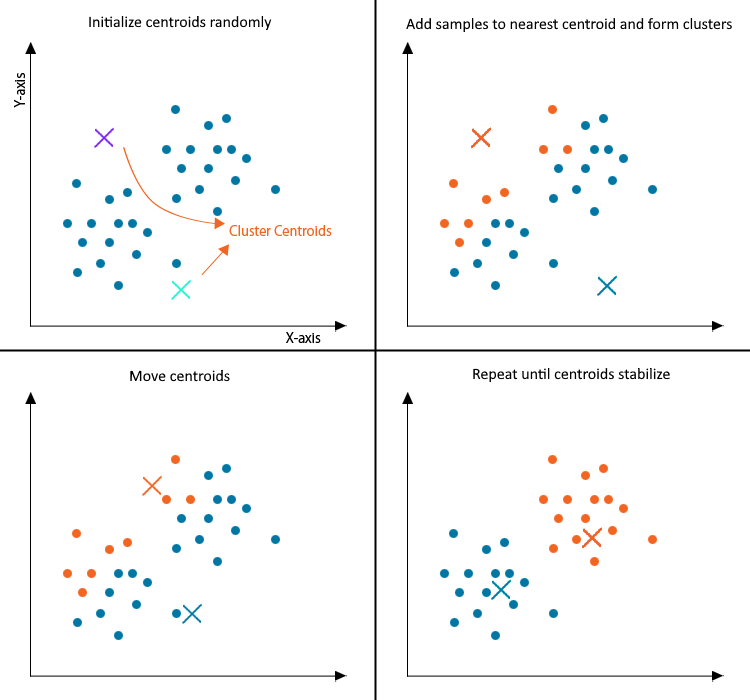
\includegraphics[width=\linewidth]{k-means_steps}
    % Place caption under the figure
    \caption{The steps of a k-means clustering algorithm.
        \cite{bib:k_means_clustering_algorithm}}
    % Label the caption to include in the list of figures
    \label{fig:k-means_steps}
\end{figure}
\end{verbatim}

renders Figure \ref{fig:k-means_steps}:

\begin{figure}
    % Define the figure file in the \includegraphics command
    % Must be relative to one of the paths
    % in the \graphicspath command at the top
    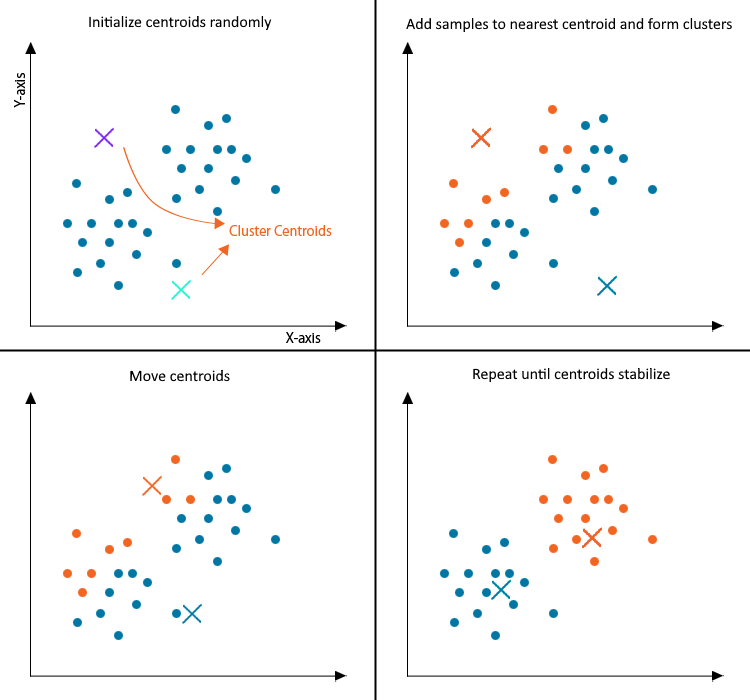
\includegraphics[width=\linewidth]{k-means_steps}
    % Place caption under the figure
    \caption{The steps of a k-means clustering algorithm.
        \cite{bib:k_means_clustering_algorithm}}
    % Label the caption to include in the list of figures
    \label{fig:k-means_steps}
\end{figure}

\backmatter

% abbreviations table
\abbreviations
\begin{center}
    \renewcommand{\arraystretch}{1.5}
    \begin{longtable}{ l @{\qquad} l }
        \toprule
        AI    & Artificial Intelligence         \\
        SPARQL & SPARQL Protocol and RDF Query Language \\
        OWL    & Web Ontology Language                  \\
        OGC    & Open Geospatial Consortium             \\
        \bottomrule
    \end{longtable}
\end{center}

% appendix
\begin{appendix}
    % mark the beginning of the appendix
    \appendixstartedtrue

    \chapter{FIRST APPENDIX}

    \chapter{SECOND APPENDIX}

    % add appendix line to ToC
    \phantomsection
    \addcontentsline{toc}{chapter}{APPENDICES}
\end{appendix}

% manually include the bibliography
\bibliographystyle{IEEEtran}
{\footnotesize \bibliography{IEEEabrv,references}}
% include it also in ToC (do sth on your own)
\addcontentsline{toc}{chapter}{REFERENCES}

\end{document}
